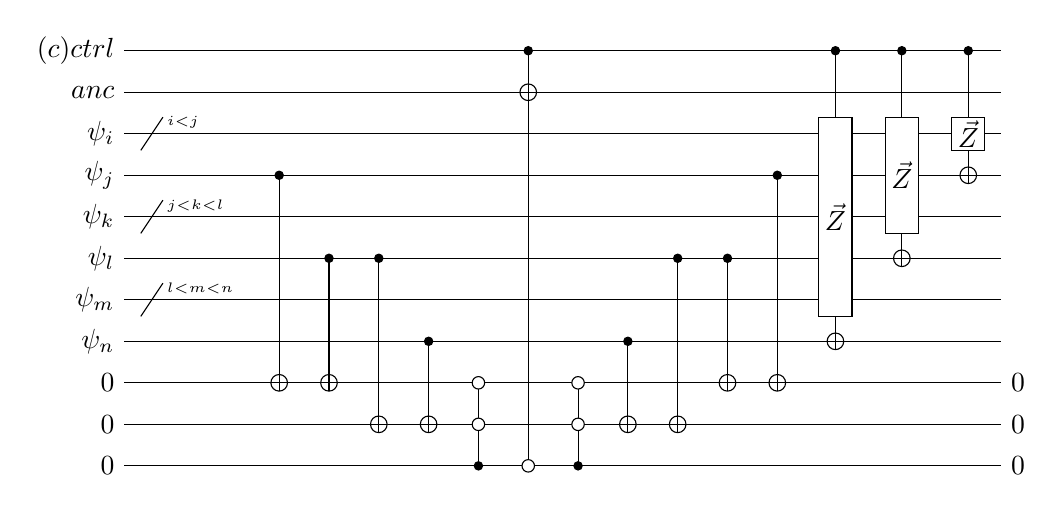
\begin{tikzpicture}[scale=1.000000,x=1pt,y=1pt]
\filldraw[color=white] (0.000000, -7.500000) rectangle (317.000000, 157.500000);
% Drawing wires
% Line 1: ctrl W \text{(c) }ctrl
\draw[color=black] (0.000000,150.000000) -- (317.000000,150.000000);
\draw[color=black] (0.000000,150.000000) node[left] {$\text{(c) }ctrl$};
% Line 2: anc W anc
\draw[color=black] (0.000000,135.000000) -- (317.000000,135.000000);
\draw[color=black] (0.000000,135.000000) node[left] {$anc$};
% Line 3: i W \psi_i
\draw[color=black] (0.000000,120.000000) -- (317.000000,120.000000);
\draw[color=black] (0.000000,120.000000) node[left] {$\psi_i$};
% Line 4: j W \psi_j
\draw[color=black] (0.000000,105.000000) -- (317.000000,105.000000);
\draw[color=black] (0.000000,105.000000) node[left] {$\psi_j$};
% Line 5: k W \psi_k
\draw[color=black] (0.000000,90.000000) -- (317.000000,90.000000);
\draw[color=black] (0.000000,90.000000) node[left] {$\psi_k$};
% Line 6: l W \psi_l
\draw[color=black] (0.000000,75.000000) -- (317.000000,75.000000);
\draw[color=black] (0.000000,75.000000) node[left] {$\psi_l$};
% Line 7: m W \psi_m
\draw[color=black] (0.000000,60.000000) -- (317.000000,60.000000);
\draw[color=black] (0.000000,60.000000) node[left] {$\psi_m$};
% Line 8: n W \psi_n
\draw[color=black] (0.000000,45.000000) -- (317.000000,45.000000);
\draw[color=black] (0.000000,45.000000) node[left] {$\psi_n$};
% Line 9: clean0 W 0 0
\draw[color=black] (0.000000,30.000000) -- (317.000000,30.000000);
\draw[color=black] (0.000000,30.000000) node[left] {$0$};
% Line 10: clean1 W 0 0
\draw[color=black] (0.000000,15.000000) -- (317.000000,15.000000);
\draw[color=black] (0.000000,15.000000) node[left] {$0$};
% Line 11: clean2 W 0 0
\draw[color=black] (0.000000,0.000000) -- (317.000000,0.000000);
\draw[color=black] (0.000000,0.000000) node[left] {$0$};
% Done with wires; drawing gates
% Line 13: i / ^{i<j}
\draw (6.000000, 114.000000) -- (14.000000, 126.000000);
\draw (12.000000, 123.000000) node[right] {$\scriptstyle{^{i<j}}$};
% Line 14: k / ^{j<k<l}
\draw (6.000000, 84.000000) -- (14.000000, 96.000000);
\draw (12.000000, 93.000000) node[right] {$\scriptstyle{^{j<k<l}}$};
% Line 15: m / ^{l<m<n}
\draw (6.000000, 54.000000) -- (14.000000, 66.000000);
\draw (12.000000, 63.000000) node[right] {$\scriptstyle{^{l<m<n}}$};
% Line 16: ctrl anc i j k l m n clean0 LABEL
% Line 17: j +clean0
\draw (56.000000,105.000000) -- (56.000000,30.000000);
\filldraw (56.000000, 105.000000) circle(1.500000pt);
\begin{scope}
\draw[fill=white] (56.000000, 30.000000) circle(3.000000pt);
\clip (56.000000, 30.000000) circle(3.000000pt);
\draw (53.000000, 30.000000) -- (59.000000, 30.000000);
\draw (56.000000, 27.000000) -- (56.000000, 33.000000);
\end{scope}
% Line 18: l +clean0
\draw (74.000000,75.000000) -- (74.000000,30.000000);
\filldraw (74.000000, 75.000000) circle(1.500000pt);
\begin{scope}
\draw[fill=white] (74.000000, 30.000000) circle(3.000000pt);
\clip (74.000000, 30.000000) circle(3.000000pt);
\draw (71.000000, 30.000000) -- (77.000000, 30.000000);
\draw (74.000000, 27.000000) -- (74.000000, 33.000000);
\end{scope}
% Line 19: l +clean1
\draw (92.000000,75.000000) -- (92.000000,15.000000);
\filldraw (92.000000, 75.000000) circle(1.500000pt);
\begin{scope}
\draw[fill=white] (92.000000, 15.000000) circle(3.000000pt);
\clip (92.000000, 15.000000) circle(3.000000pt);
\draw (89.000000, 15.000000) -- (95.000000, 15.000000);
\draw (92.000000, 12.000000) -- (92.000000, 18.000000);
\end{scope}
% Line 20: n +clean1
\draw (110.000000,45.000000) -- (110.000000,15.000000);
\filldraw (110.000000, 45.000000) circle(1.500000pt);
\begin{scope}
\draw[fill=white] (110.000000, 15.000000) circle(3.000000pt);
\clip (110.000000, 15.000000) circle(3.000000pt);
\draw (107.000000, 15.000000) -- (113.000000, 15.000000);
\draw (110.000000, 12.000000) -- (110.000000, 18.000000);
\end{scope}
% Line 21: -clean0 -clean1 clean2
\draw (128.000000,30.000000) -- (128.000000,0.000000);
\draw[fill=white] (128.000000, 30.000000) circle(2.250000pt);
\draw[fill=white] (128.000000, 15.000000) circle(2.250000pt);
\filldraw (128.000000, 0.000000) circle(1.500000pt);
% Line 22: ctrl -clean2 +anc
\draw (146.000000,150.000000) -- (146.000000,0.000000);
\filldraw (146.000000, 150.000000) circle(1.500000pt);
\draw[fill=white] (146.000000, 0.000000) circle(2.250000pt);
\begin{scope}
\draw[fill=white] (146.000000, 135.000000) circle(3.000000pt);
\clip (146.000000, 135.000000) circle(3.000000pt);
\draw (143.000000, 135.000000) -- (149.000000, 135.000000);
\draw (146.000000, 132.000000) -- (146.000000, 138.000000);
\end{scope}
% Line 23: -clean0 -clean1 clean2
\draw (164.000000,30.000000) -- (164.000000,0.000000);
\draw[fill=white] (164.000000, 30.000000) circle(2.250000pt);
\draw[fill=white] (164.000000, 15.000000) circle(2.250000pt);
\filldraw (164.000000, 0.000000) circle(1.500000pt);
% Line 24: n +clean1
\draw (182.000000,45.000000) -- (182.000000,15.000000);
\filldraw (182.000000, 45.000000) circle(1.500000pt);
\begin{scope}
\draw[fill=white] (182.000000, 15.000000) circle(3.000000pt);
\clip (182.000000, 15.000000) circle(3.000000pt);
\draw (179.000000, 15.000000) -- (185.000000, 15.000000);
\draw (182.000000, 12.000000) -- (182.000000, 18.000000);
\end{scope}
% Line 25: l +clean1
\draw (200.000000,75.000000) -- (200.000000,15.000000);
\filldraw (200.000000, 75.000000) circle(1.500000pt);
\begin{scope}
\draw[fill=white] (200.000000, 15.000000) circle(3.000000pt);
\clip (200.000000, 15.000000) circle(3.000000pt);
\draw (197.000000, 15.000000) -- (203.000000, 15.000000);
\draw (200.000000, 12.000000) -- (200.000000, 18.000000);
\end{scope}
% Line 26: l +clean0
\draw (218.000000,75.000000) -- (218.000000,30.000000);
\filldraw (218.000000, 75.000000) circle(1.500000pt);
\begin{scope}
\draw[fill=white] (218.000000, 30.000000) circle(3.000000pt);
\clip (218.000000, 30.000000) circle(3.000000pt);
\draw (215.000000, 30.000000) -- (221.000000, 30.000000);
\draw (218.000000, 27.000000) -- (218.000000, 33.000000);
\end{scope}
% Line 27: j +clean0
\draw (236.000000,105.000000) -- (236.000000,30.000000);
\filldraw (236.000000, 105.000000) circle(1.500000pt);
\begin{scope}
\draw[fill=white] (236.000000, 30.000000) circle(3.000000pt);
\clip (236.000000, 30.000000) circle(3.000000pt);
\draw (233.000000, 30.000000) -- (239.000000, 30.000000);
\draw (236.000000, 27.000000) -- (236.000000, 33.000000);
\end{scope}
% Line 29: i j k l m G $\vec{Z}$ ctrl +n
\draw (257.000000,150.000000) -- (257.000000,45.000000);
\begin{scope}
\draw[fill=white] (257.000000, 90.000000) +(-45.000000:8.485281pt and 50.911688pt) -- +(45.000000:8.485281pt and 50.911688pt) -- +(135.000000:8.485281pt and 50.911688pt) -- +(225.000000:8.485281pt and 50.911688pt) -- cycle;
\clip (257.000000, 90.000000) +(-45.000000:8.485281pt and 50.911688pt) -- +(45.000000:8.485281pt and 50.911688pt) -- +(135.000000:8.485281pt and 50.911688pt) -- +(225.000000:8.485281pt and 50.911688pt) -- cycle;
\draw (257.000000, 90.000000) node {$\vec{Z}$};
\end{scope}
\filldraw (257.000000, 150.000000) circle(1.500000pt);
\begin{scope}
\draw[fill=white] (257.000000, 45.000000) circle(3.000000pt);
\clip (257.000000, 45.000000) circle(3.000000pt);
\draw (254.000000, 45.000000) -- (260.000000, 45.000000);
\draw (257.000000, 42.000000) -- (257.000000, 48.000000);
\end{scope}
% Line 30: i j k G $\vec{Z}$ ctrl +l
\draw (281.000000,150.000000) -- (281.000000,75.000000);
\begin{scope}
\draw[fill=white] (281.000000, 105.000000) +(-45.000000:8.485281pt and 29.698485pt) -- +(45.000000:8.485281pt and 29.698485pt) -- +(135.000000:8.485281pt and 29.698485pt) -- +(225.000000:8.485281pt and 29.698485pt) -- cycle;
\clip (281.000000, 105.000000) +(-45.000000:8.485281pt and 29.698485pt) -- +(45.000000:8.485281pt and 29.698485pt) -- +(135.000000:8.485281pt and 29.698485pt) -- +(225.000000:8.485281pt and 29.698485pt) -- cycle;
\draw (281.000000, 105.000000) node {$\vec{Z}$};
\end{scope}
\filldraw (281.000000, 150.000000) circle(1.500000pt);
\begin{scope}
\draw[fill=white] (281.000000, 75.000000) circle(3.000000pt);
\clip (281.000000, 75.000000) circle(3.000000pt);
\draw (278.000000, 75.000000) -- (284.000000, 75.000000);
\draw (281.000000, 72.000000) -- (281.000000, 78.000000);
\end{scope}
% Line 31: i G $\vec{Z}$ ctrl +j
\draw (305.000000,150.000000) -- (305.000000,105.000000);
\begin{scope}
\draw[fill=white] (305.000000, 120.000000) +(-45.000000:8.485281pt and 8.485281pt) -- +(45.000000:8.485281pt and 8.485281pt) -- +(135.000000:8.485281pt and 8.485281pt) -- +(225.000000:8.485281pt and 8.485281pt) -- cycle;
\clip (305.000000, 120.000000) +(-45.000000:8.485281pt and 8.485281pt) -- +(45.000000:8.485281pt and 8.485281pt) -- +(135.000000:8.485281pt and 8.485281pt) -- +(225.000000:8.485281pt and 8.485281pt) -- cycle;
\draw (305.000000, 120.000000) node {$\vec{Z}$};
\end{scope}
\filldraw (305.000000, 150.000000) circle(1.500000pt);
\begin{scope}
\draw[fill=white] (305.000000, 105.000000) circle(3.000000pt);
\clip (305.000000, 105.000000) circle(3.000000pt);
\draw (302.000000, 105.000000) -- (308.000000, 105.000000);
\draw (305.000000, 102.000000) -- (305.000000, 108.000000);
\end{scope}
% Done with gates; drawing ending labels
\draw[color=black] (317.000000,30.000000) node[right] {$0$};
\draw[color=black] (317.000000,15.000000) node[right] {$0$};
\draw[color=black] (317.000000,0.000000) node[right] {$0$};
% Done with ending labels; drawing cut lines and comments
% Done with comments
\end{tikzpicture}
